\section{Einfache Impulse}
\subsection{Rechteckimpuls/ -funktion \texorpdfstring{$rect_T\left(t\right)$}{}}
\begin{multicols}{2}
\begin{equation*}
x\left(t\right) = X_0 \cdot rect_T\left(t\right) 
\end{equation*}

\begin{itemize}
 \item T: Rechteckimpulsbreite \(> 0\)
 \item an den Sprungstellen nimmt der Impuls die Hälfte des max. Wertes an
\end{itemize}

\begin{center}
 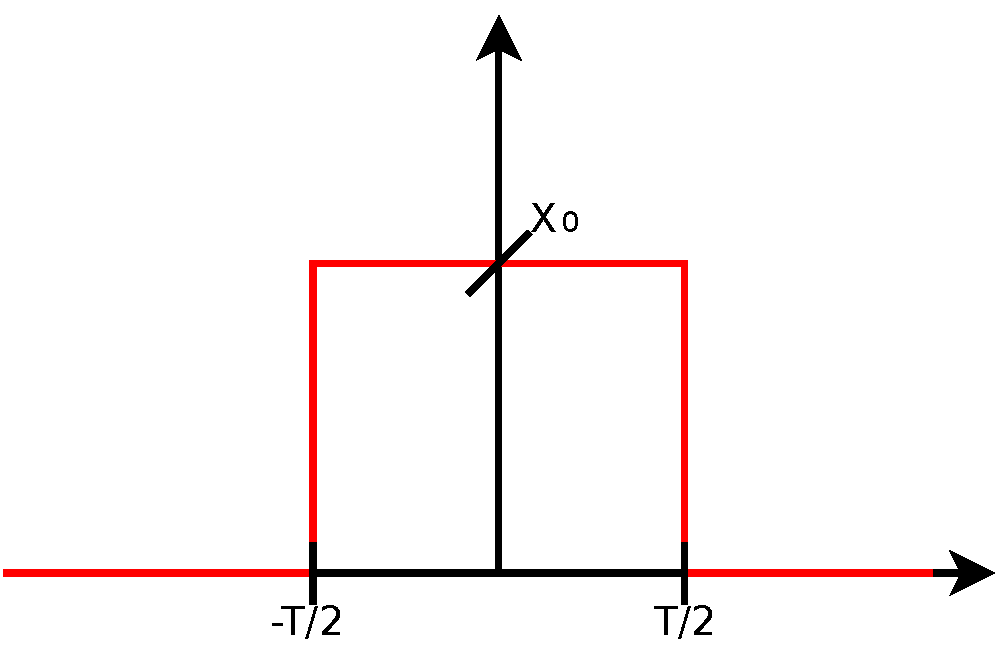
\includegraphics[width=50mm,keepaspectratio=true]{./Elektrotechnik/Bilder/rect.pdf}
\end{center}

\end{multicols}

\subsection{Dreiecksimpuls/ -funktion \texorpdfstring{$\Lambda_T\left(t\right)$}{}}
\begin{multicols}{2}
 \begin{align*}
x\left(t\right) &= X_0 \cdot \Lambda_T\left(t\right) \\
\Lambda_T\left(t\right) &=\begin{cases}
1-\left|t/T\right| \text{ für } \left|t\right| < T\\
0 \text{ für } \left|t\right| > T
\end{cases}
\end{align*}

\begin{itemize}
 \item T: Dauer einer ansteigenden / abfallenden Flanke
\end{itemize}

\begin{center}
 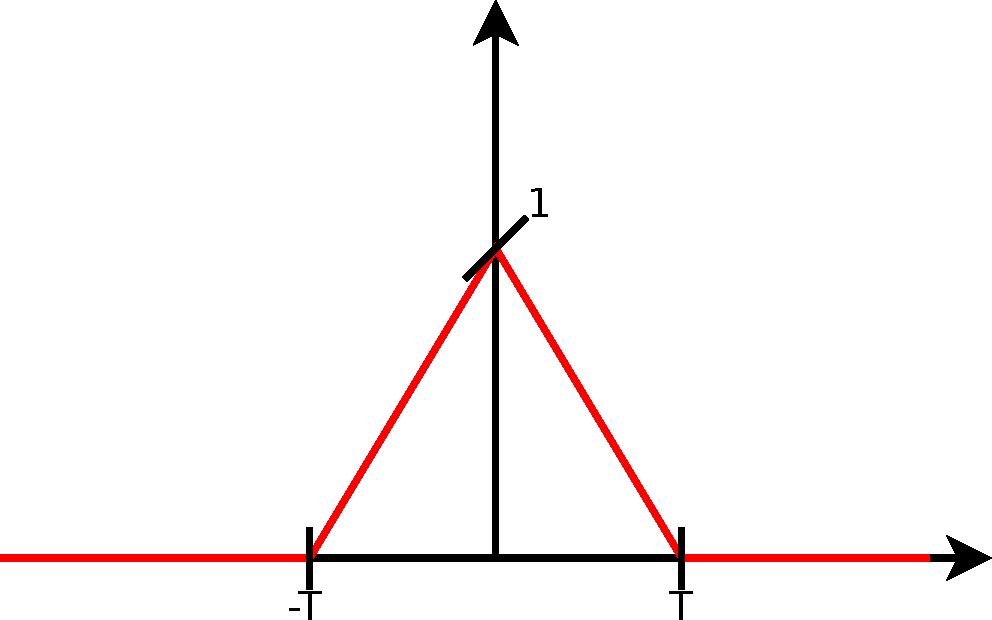
\includegraphics[width=50mm,keepaspectratio=true]{./Elektrotechnik/Bilder/lambda.pdf}
\end{center}

\end{multicols}

\section{Elementare Operationen auf zeitliche Verläufe}
\subsection{Beeinflußung der Ordinate}

\begin{multicols}{2}
 \subsubsection*{Signaloffset \texorpdfstring{$X_{OFFS}$}{}}
  \begin{equation*}
   x_{neu}\left(t\right) = x_{alt}\left(t\right) + X_{OFFS} 
  \end{equation*}
\vfill
  \begin{center}
  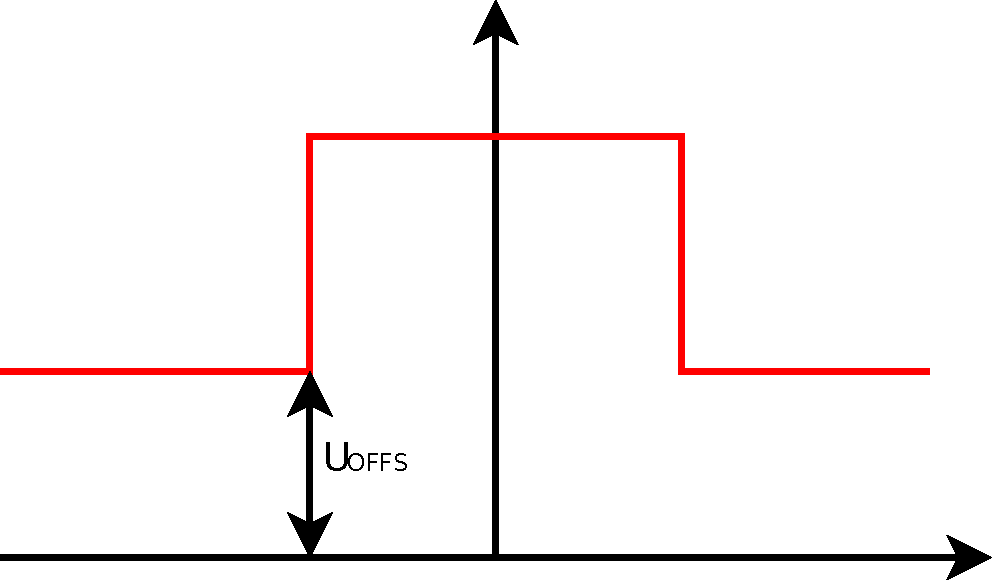
\includegraphics[width=50mm,keepaspectratio=true]{./Elektrotechnik/Bilder/uoffs.pdf}
  \end{center}
\end{multicols}

\begin{multicols}{2}
 \subsubsection*{Skalierungsfaktor \texorpdfstring{$V \left(V \neq 0 \right) $}{}}
  \begin{equation*}
   x_{neu}\left(t\right) = V \cdot x_{alt}\left(t\right) 
  \end{equation*}
\vfill
  \begin{center}
  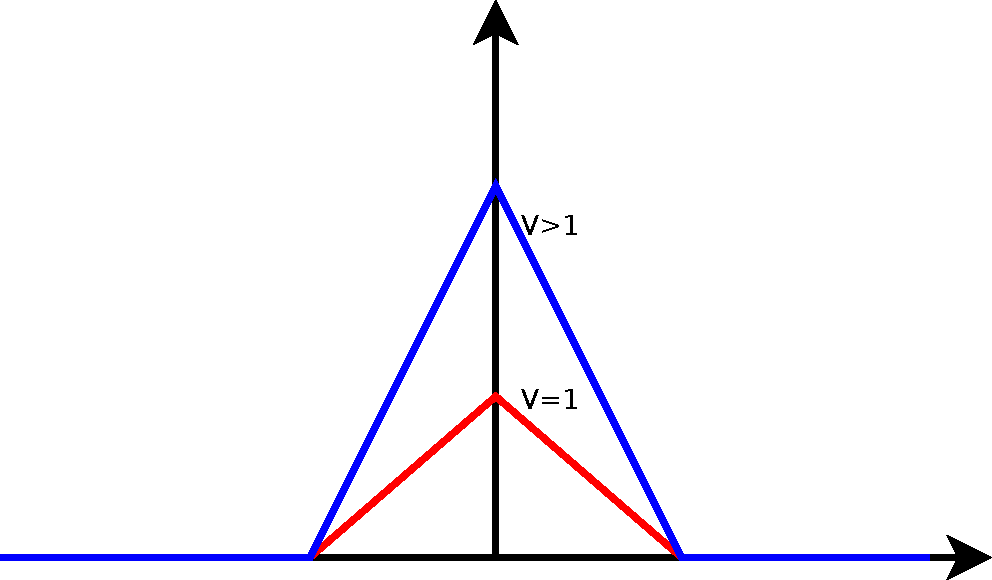
\includegraphics[width=50mm,keepaspectratio=true]{./Elektrotechnik/Bilder/skalierung.pdf}
  \end{center}
\end{multicols}

\subsection{Beeinflußung der Abszisse}
\begin{multicols}{2}
 \subsubsection{zeitliche Verschiebung \texorpdfstring{$t_0$}{}}
  \begin{equation*}
   x_{neu}\left(t\right) = x_{alt}\left(t - t_0\right) \text{ mit } t_0 = const.
  \end{equation*}
  \begin{itemize}
   \item Zusammenfassung der Offsetbehafteten Zeit \(t - t_0\) zu einer neuen Zeitbasis \(\tau = t - t_0\)
   \item \(x_{neu}\left(\tau + t_0\right) = x_{alt}\left(\tau\right) \) \\
         \(t > 0\) Verschiebung nach rechts\\
	 	 \(t < 0\) Verschiebung nach links
  \end{itemize}
\vfill
  \begin{center}
  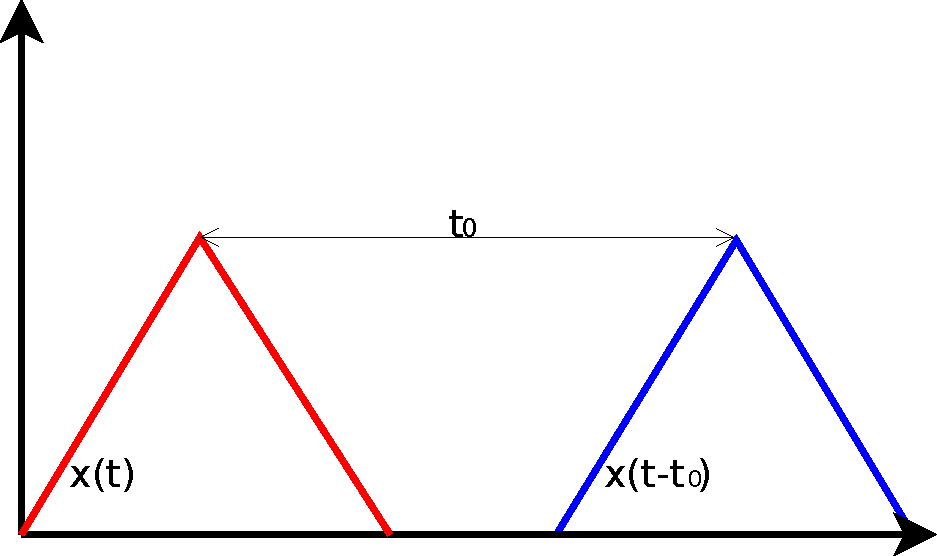
\includegraphics[width=50mm,keepaspectratio=true]{./Elektrotechnik/Bilder/zeitbasis.pdf}
  \end{center}
  \vspace*{2mm}
\end{multicols}

\begin{multicols}{2}
 \subsubsection{Negation des Arguments \texorpdfstring{$t$}{}}
  \begin{align*}
   x_{neu}\left(t\right) &= x_{alt}\left(-t\right) \text{ mit } \tau = -t \\
   x_{neu}\left(-\tau\right) &= x_{alt}\left(\tau\right)
  \end{align*}
  \begin{itemize}
   \item gleiche Funktionswerte mit negierter Zeitbasis, somit Spiegelung an der Ordinate
  \end{itemize}

\vfill
  \begin{center}
  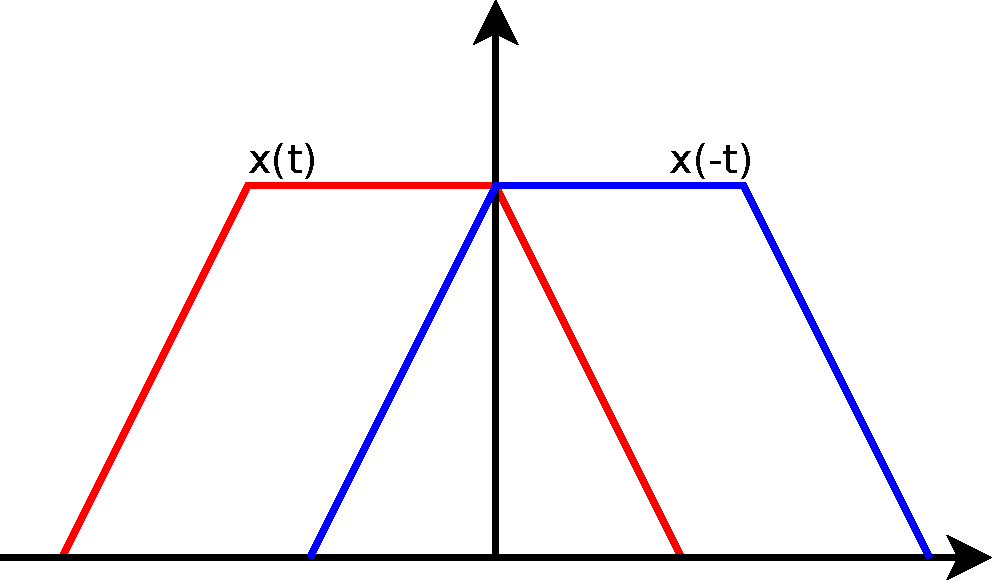
\includegraphics[width=50mm,keepaspectratio=true]{./Elektrotechnik/Bilder/argument.pdf}
  \end{center}
\end{multicols}

\begin{multicols}{2}
\subsubsection*{Nagation des Arguments \texorpdfstring{$t$}{} \\ sowie eine Verschiebung um \texorpdfstring{$t_0$}{}}
\begin{align*}
  &x_{neu}\left(t\right) = x_{alt}\left(t_0 - t\right) \\
  &\text{ mit } t_0 = const.\\
  &x_{neu}\left(t\right) = x_{alt}\left(\tau + 1/2 t_0\right)\\
  &x_{neu}\left(1/2 t_0 - \tau\right) = x_{alt}\left(\tau + 1/2 t_0\right)\\
\end{align*}
\vfill
\begin{center}
 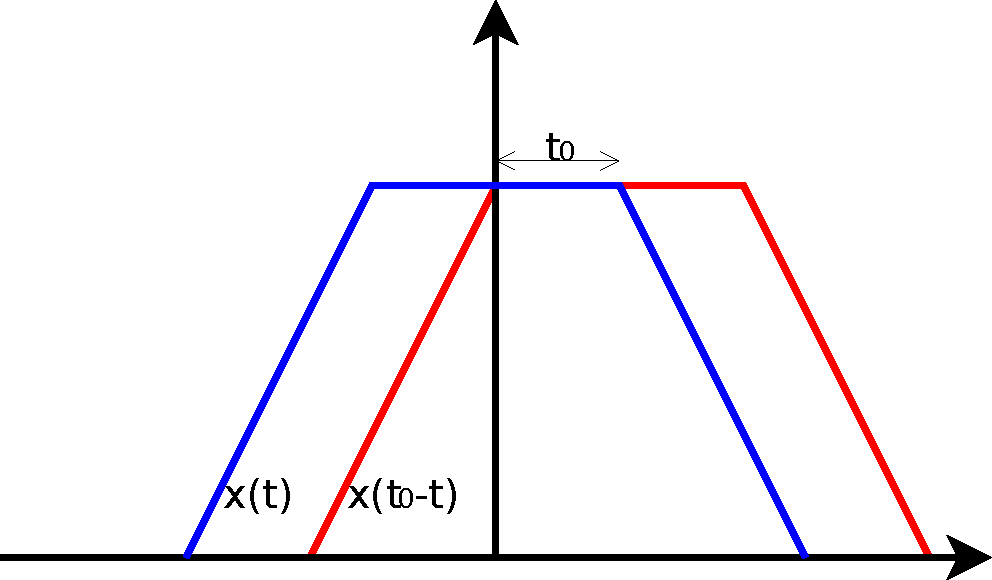
\includegraphics[width=50mm,keepaspectratio=true]{./Elektrotechnik/Bilder/argumentversch.pdf}
\end{center}

\end{multicols}
\begin{itemize}
 \item neue Zeitbasis \(\tau + 1/2 t_0\)
 \item gleiche Funktionswerte, gespiegelt an der Senkrechten von \(1/2 t_0\)
\end{itemize}

\subsubsection*{Skalierungsfaktor \texorpdfstring{$a \neq 0$}{}}
\begin{multicols}{2}
\begin{align*}
  &x_{neu}\left(t\right) = x_{alt}\left(a \cdot t\right) \\
  &\text{ mit } a = const.\\
  &x_{neu}\left(t\right) = x_{alt}\left(\tau\right)\\
  &x_{neu}\left(\tau / a\right) = x_{alt}\left(\tau\right)
\end{align*}
\vfill
\begin{center}
 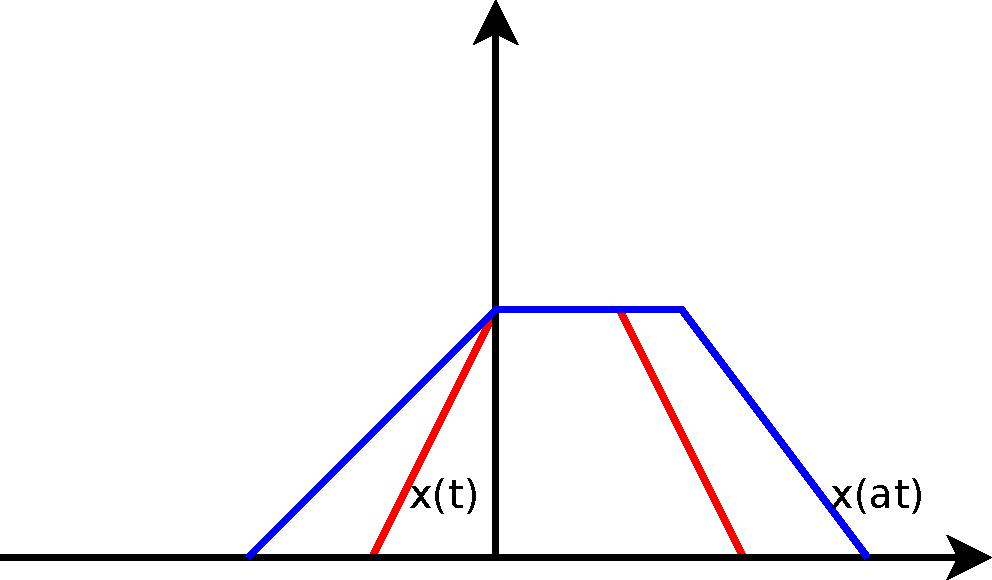
\includegraphics[width=50mm,keepaspectratio=true]{./Elektrotechnik/Bilder/skalierungsfaktor.pdf}
\end{center}

\end{multicols}
\begin{itemize}
 \item neue Zeitbasis \(\tau = a \cdot t\)
 \item gleiche Funktionswerte, wenn die Zeitbasis durch \(a\) geteilt wird
 \item \(a > 1\) Funktion wird gestaucht\\
       \(0 < a < 1\) Funktion wird gestreckt 
\end{itemize}

\subsection{Einheitssprungfunktion / Deltaimpuls}
\subsubsection*{angenäherte Einheitssprungfunktion
\texorpdfstring{$\tilde{\sigma}\left(t, \epsilon \right)$}{}}
\begin{multicols}{2}
 \begin{itemize}
  \item endlicher Geradenanstieg
  \item Endwert von 1
 \end{itemize}
\vfill
\begin{center}
 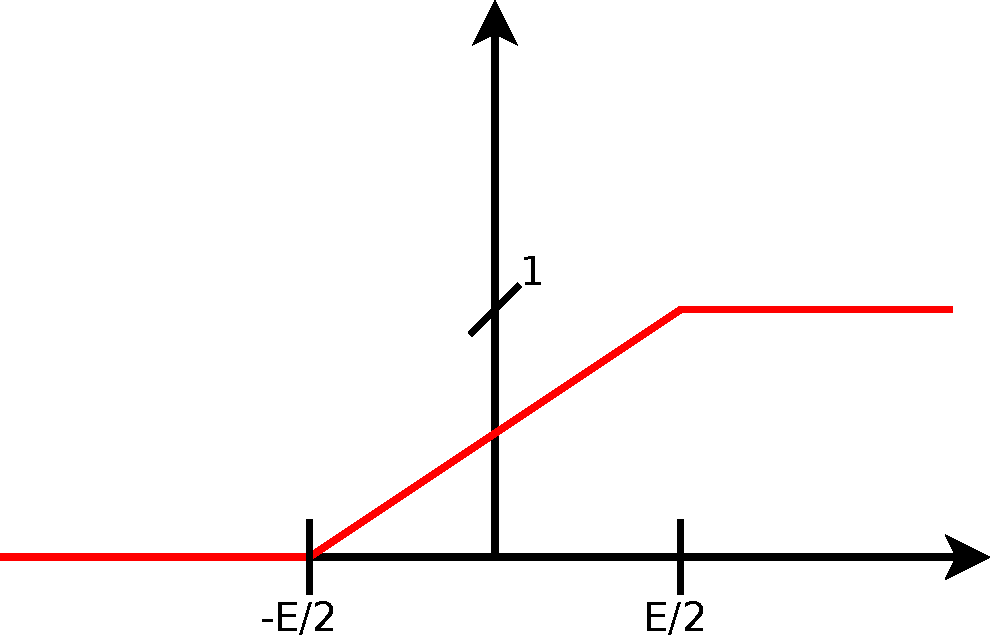
\includegraphics[width=50mm,keepaspectratio=true]{./Elektrotechnik/Bilder/einheitssprungang.pdf}
\end{center}
\vfill
\end{multicols}

\subsubsection*{Einheitsimpuls / Deltaimpuls
\texorpdfstring{$\tilde{\delta}\left(t, \epsilon\right)$}{}}
\begin{multicols}{2}
\begin{itemize}
  \item Fläche des Impulses ist 1
  \item Impulshöhe und Breite variabel
\end{itemize}
\vfill
\begin{center}
	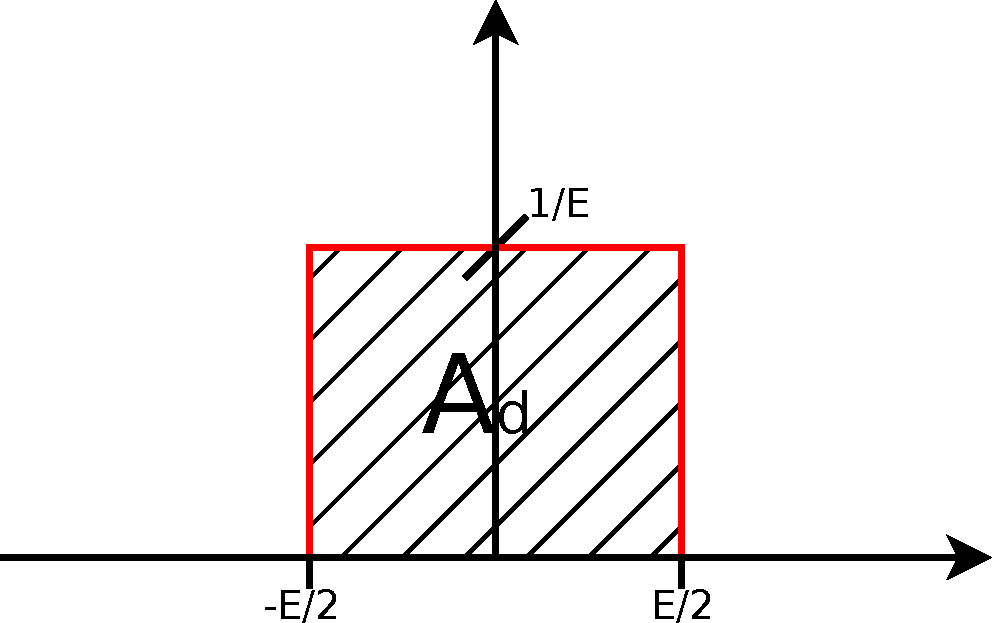
\includegraphics[width=50mm,keepaspectratio=true]{./Elektrotechnik/Bilder/einheitsimpuls.pdf}
\end{center}
\vfill
\end{multicols}


Mathematischer Zusammenhang:
\[
\tilde{\delta} \left(t, \epsilon \right) = \frac{d \tilde{\sigma} \left( t,
\epsilon \right)}{dt} \quad \leftrightarrow \quad \tilde{\sigma} \left( t,
\epsilon \right) = \int_{-\infty}^{t} \tilde{\delta} \left( t, \epsilon \right) dt
\]
Beim Grenzübergang \( \epsilon \rightarrow 0 \) ergibt die
Einheitssprungfunktion \( \sigma \left( t \right) \) bzw. deren Ableitung den
Deltaimpuls \( \delta \left( t \right) \).
\begin{multicols}{2}
\vfill
\[
\delta\left(t\right) = \frac{d \sigma \left(t\right)}{dt} = 
\begin{cases}
+ \infty \text{ für } t = 0 \\
\\
0 \text{ für } t \neq 0
\end{cases}
\]
\vfill
\[
\sigma \left(t\right) = \int_{-\infty}^{t} \delta \left(t\right)dt = 
\begin{cases}
1 \text{ für } t > 0\\
\frac{1}{2} \text{ für } t = 0\\
0 \text{ für } t < 0\\
\end{cases}
\]
\vfill
\end{multicols}

